\chapter{Appendix}

\section{First Stage Regressions and Relevance condition}
\label{section:appendix_rank}
This sections shows the details of the first stage for our IV strategies. The following regressions have as dependent variable experience and as independent variable a binary indicator of close experience, which is the instrument throughtout the paper. The following IV regressions have a first stage which is showed in the corresponding table. Note all F-statistics are significant at p<0.01.

\begin{enumerate}
  \item Main results section: Table \ref{tab:table_F_main_exp1} (rolling experience) and Table \ref{tab:table_F_main_exp2} (annualized cumulative).
  \item Standarized bids section: Table \ref{tab:table_F_bids}.
  \item Quality section: Table \ref{tab:table_F_quality}.
\end{enumerate}


\input{C:/repos/learn-doing/thesis/tables/table_F_main_exp1.txt}

\input{C:/repos/learn-doing/thesis/tables/table_F_main_exp2.txt}

\input{C:/repos/learn-doing/thesis/tables/table_F_bids.txt}

\input{C:/repos/learn-doing/thesis/tables/table_F_quality.txt}


\clearpage
\section{Additional Sample Characterization}
This section expands on the sample characterization of the Data chapter. Regional and market participants descriptions are included in the form of tables or graphs.

\subsection{Regional Representation}
\input{C:/repos/learn-doing/thesis/tables/sampleregion.txt}
\clearpage

\subsection{Top Market Participants}
\input{C:/repos/learn-doing/thesis/tables/topgov.txt}
\small
\input{C:/repos/learn-doing/thesis/tables/topfirms.txt}


\clearpage


\section{Bids and Winning Probability}
This section explores the relationship between bids and winning probability. We develop two simple regressions of the form:
\begin{equation}
  \label{eqn:helpbids}
INDWIN_{ij}  = \alpha +BID_{ij}+  FIRSTYEAR_{ij}+X_j\varepsilon_{ij}
\end{equation}
Where $INDWIN$ is an indicator for winning the firm $i$ submitting a winning bid for contract $j$, $BID$ is a standarized bid, and $X_j$ are controls for the contract. In the first specification, $X_j$ are just fixed effects for Year and Region. In the second specification, we employ per-contract Fixed Effects, which means that we identify the parameter of interest through the variation in bids and outcomes for the participants in the same auction. The second specification omits the intercept as well.

Our sample consists in contracts for which i) there were two or more valid participants and ii) had a winner chosen. This renders 29,608 observations. The regressions are at the firm-bid level.

Results are shown in Table \ref{tab:table_bids_help}. Notably, the results imply that a three percentage point decrease in the standarize bid is correlated with an increase of ten percentage points in winning probability. Given that previous discussions showed that price is an awarding component in most contracts, there seems to be enough basis to establish a causal nexus between submitting lower bids and winning contracts, altough there is still much uncertainty about the actual magnitude. For similar  example, probably all firms' measures of quality are probably correlated, so we cannot attribute the win to smaller bids alone.

\input{C:/repos/learn-doing/thesis/tables/table_bids_help.txt}

\clearpage
\section{ELO algorithm : theory and implementation}
\label{section:eloappendix}
\subsection{Introduction}\footnote{This section is based on Arpad Elo's book introduction to the Elo system in \citep{elo1978rating}}
The Elo Ranking is a system to place players in a numerical rating scale, in which differences among players can be converted into scoring or winning probabilities. Similarly, scoring percentages (over time or competitions) can be converted into ranking differences. Ratings in the Elo system are points in a scale which, for historical reasons, has been chosen to have its midpoint at 2000. However, the importance is on difference of ratings rather than in absolute number, since a Elo ranking is only valid within a specific pool of players.

The first basic principle of the Elo system is that performances from an individual are normally distributed, when evaluated on an appropriate scale. Let the expectancy score be the expected number of points that a player is expected to win, out of the total possible, in a match or matches. According to Elo, the percentage expectancy score for a player is a function of the difference in rating with the opponent. For example, a player one standard deviation in ranking above another has an approximate  percentage expectancy score. This follows from a standard computation of the probability that a draw from a random variable of mean $\mu_1$ and standard deviation $\sigma$ is higher than a random variable of mean $\mu_2$ and standard deviation $\sigma$ as well.

The performance of a player is evaluated on the basis of how do his or her actual performance compare to the expected score, both of his own and his opponents. The \textit{Perfomance Rating} is a measure of performance evaluated over a number of encounters which combines the average rating of the competition and the percent score achieved. A more stable measure over time is the \textit{Player rating} which ought to vary less than the performance rating. In the context of chess, where it was developed, a performance rating would be obtained for a chess tournament, while the rating of the player would be his overall ranking. The player rating can be updated periodically through Performance Ratings as follows.

Over intervals, rankings for players can be calculated using the Performance Rating formula:
\begin{equation}
  R_p=R_c+D_p
  \label{ratingdiscrete}
\end{equation}
Where $R_p$ is the performance rating, $R_c$ is the average rating and $D_p$ is the difference based on the percentage score $P$, which is obtained from the curve or table. This formula can be employed to update rankings over periods of time. However, to maintain a continuous ranking (i.e. at every point in time), the following formula is used:
\begin{equation}
  R_n=R_0 + K(W-W-_e)
  \label{ratingcontinuous}
\end{equation}
Where $R_n$ is the rating after the event, $R_0$ is the rating pre-event, $K$ is the rating point value of a single game score, $W$ is the actual game score, and $W_e$ is the expected game score based on $R_0$. The parameter $K$ adjusts the relative weight of newer and older performances. A higher $K$ gives a higher weight to newer performances, and vice versa.

\subsection{Current Implementation}
The algorithm employed in the current investigation is a modified  Elo system suited for multiplayer games with variable player numbers. The implementation used is contained the function $elom$ of the R package \textit{PlayerRatings}, which implements several types of ranking algorithms \citep{stephenson2020package}. The adaptation of the canonical Elo algorithm to allow for a variable number of (multiple) players requires to i) implement a computation of expected scores that considers the wider range of competitors, and ii) change the way points are awarded and substracted depending on the actual number of players for a game.

For algorithmic purposes, we consider a win as being awarded a contract and a lose as bidding for but not winning a specific contract. All losing players are considered "tied" in their loss, so base points substracted are the same. However, actual points substracted might differ depending on the expected score, as shown in Equation \ref{eqn:ratingadjust}.

The initial rating of a player was chosen to be 1,500. Also, since an adaptation time is needed to construct a reliable average rank, for all the analysis employing the ranking measure the first year of the data is discarded (after constructing the ranks). The documentation of the implemented algorithm recommends to make it so the net number of awarded points after a game is zero. Although keeping this recommendation and keeping the same number of points for every contest constant is impossible, we choose awarded and subtracted points such that this is true for the average contract\footnote{It would be possible the assign scores based on number of players in the contest. However, for parsimony and ease of validation purposes we take the approach to fix constant the scores.}.

To construct the ranking, the following computation steps were performed:
\begin{enumerate}[itemsep=1pt]
  \item The data was filtered to contain only contracts for which there were two or more opponents and which had a winner contractor. This renders approx. 29,000 contracts.
  \item The relevant competition datasets were constructed. In these datasets, every observation is an auction with two or more players. Columns are participants. The columns contain the names of the participants in the auction. A similar dataset contains the outcomes for each player participating.
  \item The ranking algorithm was run with the match history as the key input.
\end{enumerate}
Results consists in a ranking for every firm at every contract in the sample constructed in point 2. For interpretation purposes, rankings for contracts filtered out from the main sample are filled by i) getting the ranking of the closest past contract which performed a ranking update or ii) imputing the base rank, for contractors who did not have any contracts with ranking updates. The latter can happen if a contractor bids only in contracts where he is the only bidder \footnote{Note that for instrument construction, any contract with an imputed ranking cannot, by definition, be labeled as a close win, since this requires two or more players and a winner as a necessary condition}.

Later, in the main estimation step, the rankings are employed to identify close wins, as described in the empirical strategy section. Note that the algorithm itself employs the assumption that, for (two) equally ranked opponents, winning chances are 50 - 50. Wins against close opponents are thus attributed in both schemes mainly to random factors.

\subsection{Analysis of algorithm results}
In this section we describe some of the results to validate and interpret the rankings obtained. Figure \ref{fig:rankings_nums} shows the progression of ranks over the history of firms. Every panel is the distribution of firms at a point in their bidding history. For example, panel two shows the distribution of ranks between firms who are bidding for the second time. Note that ranks split in two after the first bidding by the win or a lose. Successive biddings "fill in" the gaps. Given that points awarded for wins are more than points substracted by loses, the distributions are right-skewed.

\begin{figure}[H]
\centering
  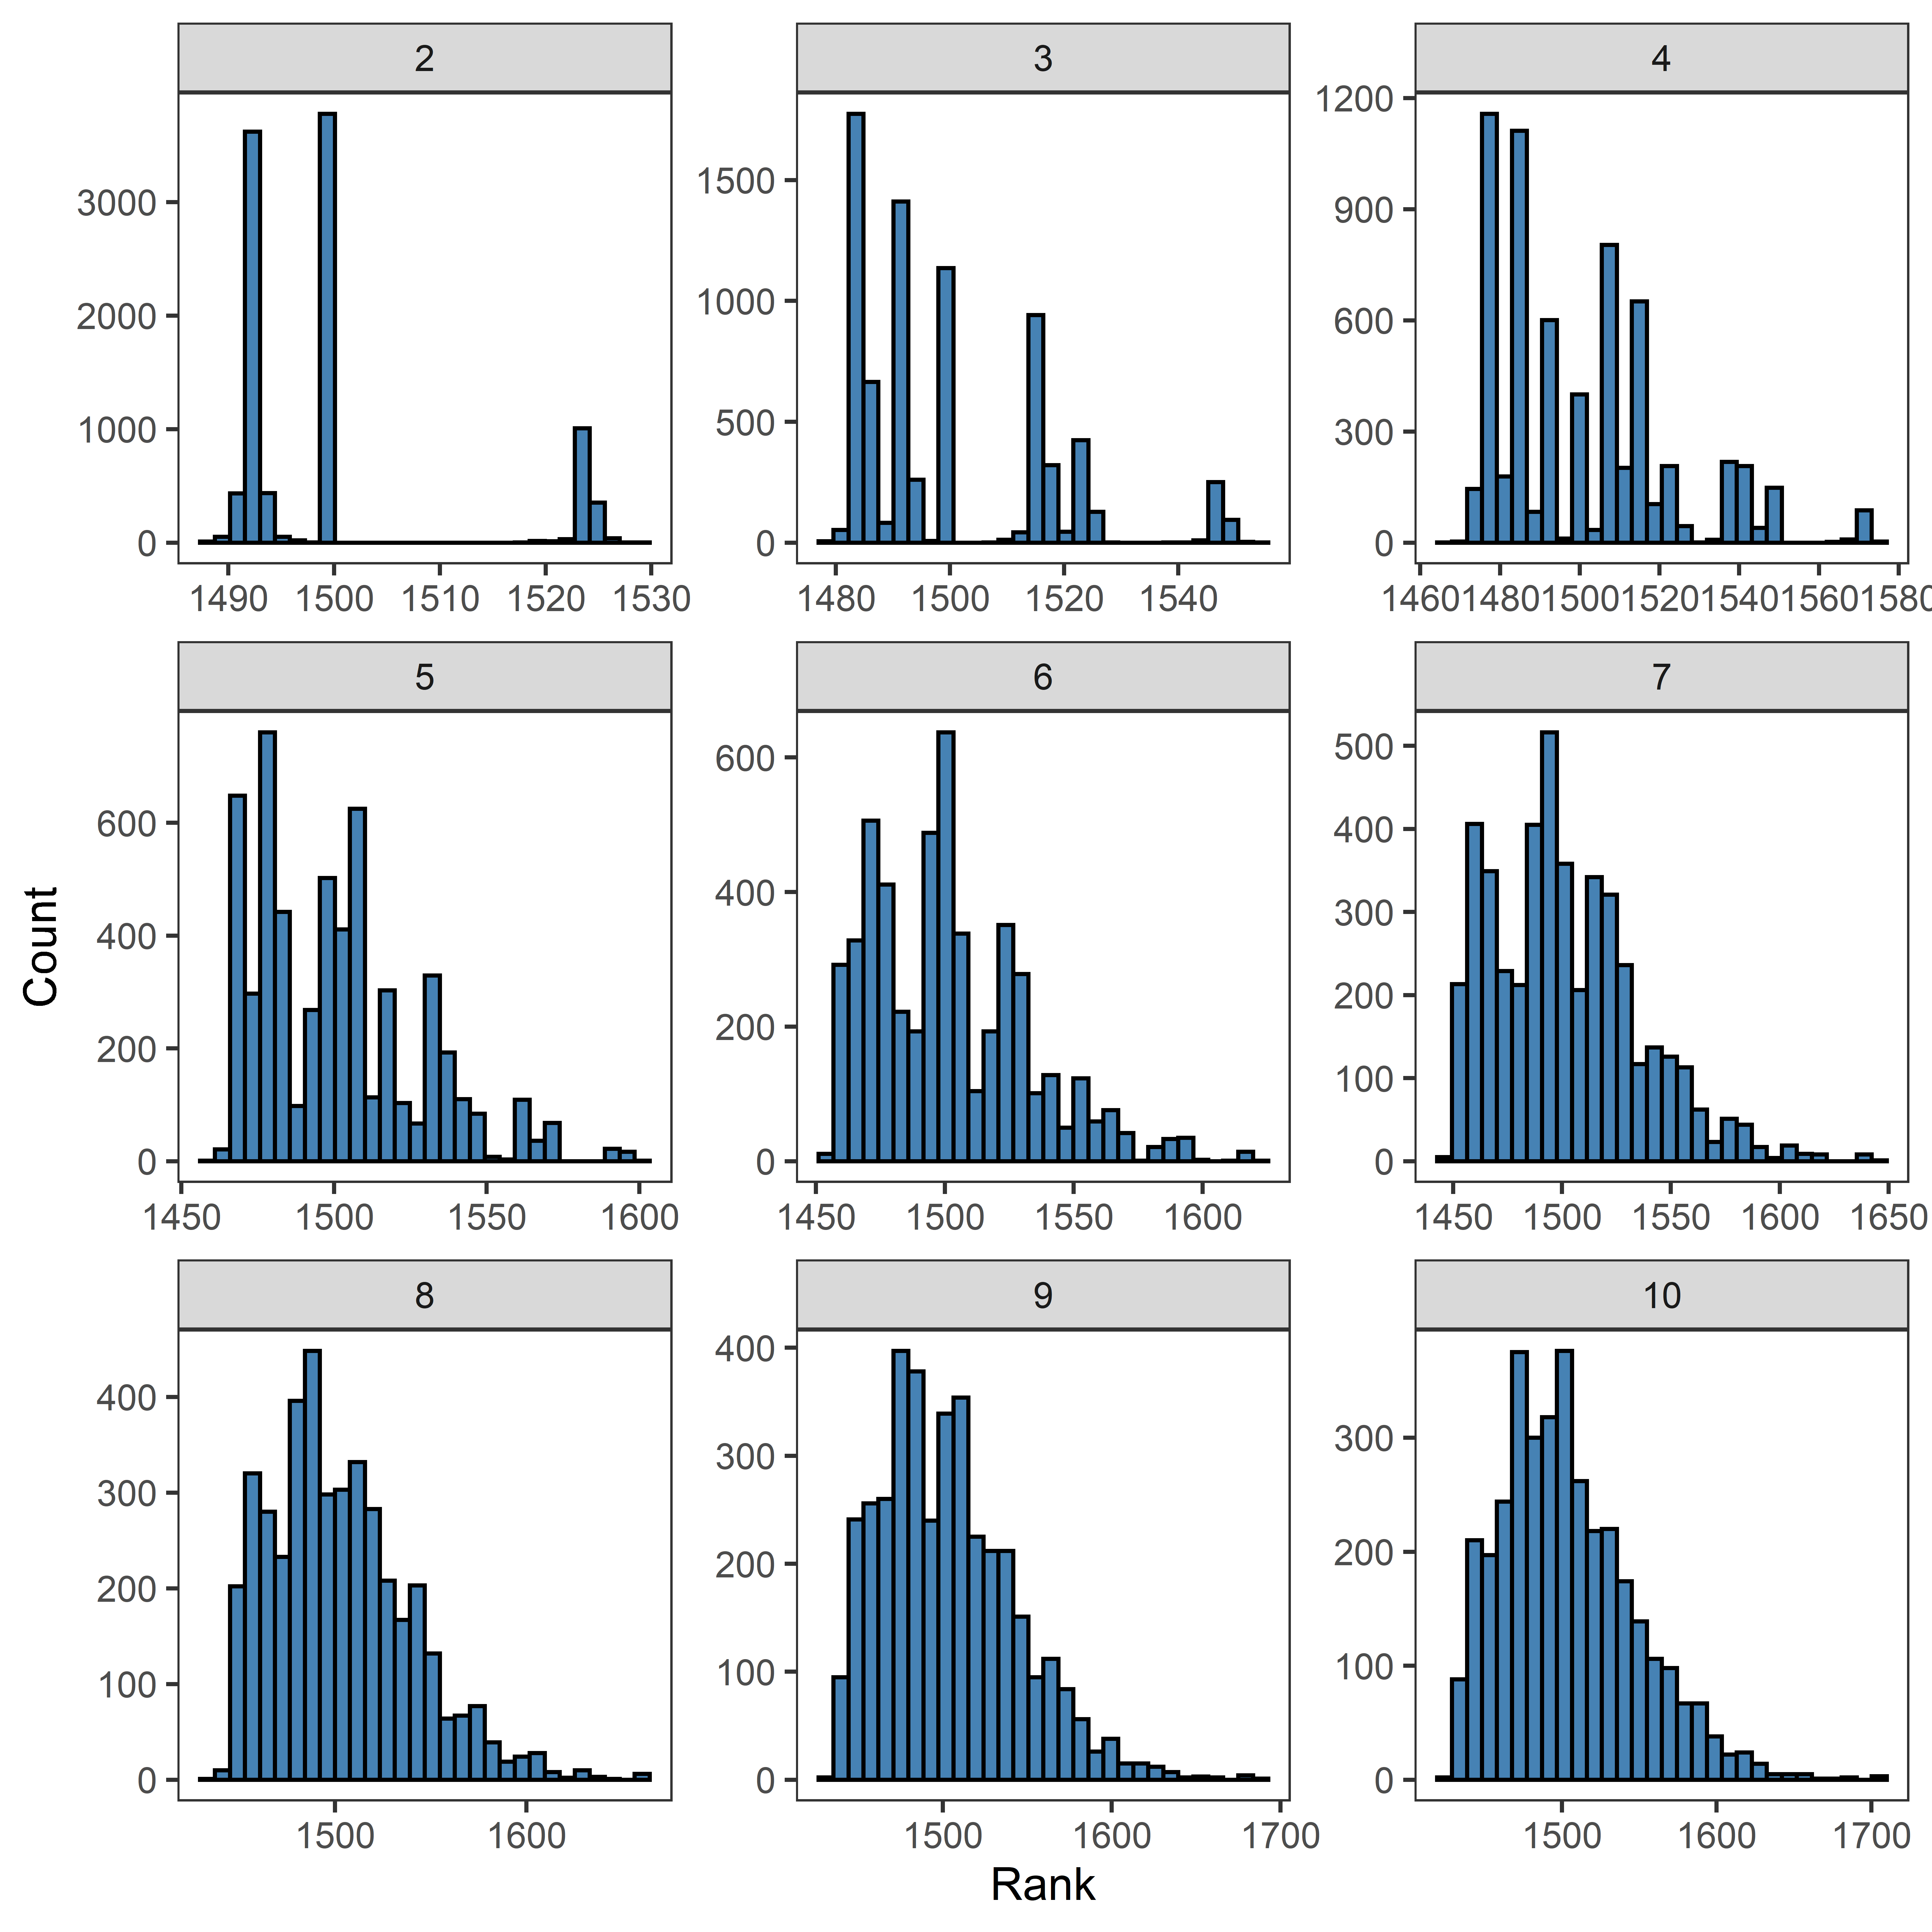
\includegraphics[scale=0.9]{rankings_nums}
  \caption{Rank progression over firm's bidding history \\ \footnotesize \underline{Note}: each panel contains the firms bidding for their $i$-th contract. The graph only displays the ranks for the first 10 bidding events. Ranks displayed are ranks $previous$ to the contract, i.e. they are not adjusted by the outcome of the i-th bidding event.}
  \label{fig:rankings_nums}
\end{figure}

The progression of rankings over time is further illustrat ed with two firms which end higher and lower respectively in ranking than their starting points at 1,500. We call the first firm "A" and the second firm "B".  The next tables show the contracts participated in, the ranking at each contract, the average ranking of opponents, the result of the bidding (i.e. win or lose) and the net effect of the "game" of the firm's ranking (measured in points). Table \ref{tab:rank_example_1} shows a firm which won all but its last contracts. While all winning contracts resulted in points added to ranking, the first wins rendered more points, as the advantage of the firm was lower. Table \ref{tab:rank_example_2} shows firm B, which mostly experienced defeats. Note that points substracted by losing are less than the ones granted for winning, so the ranking still remains close to 1,500. Also, this firm faced similar opponents, as measured by the similar average ranks.

\input{C:/repos/learn-doing/thesis/tables/rank_example_1.txt}

\input{C:/repos/learn-doing/thesis/tables/rank_example_2.txt}
\clearpage
\section{Institutional framework of types of construction projects found in the dataset}
\label{section:app_insti}
Our sample is obtained by extracting observations which belong to the category of "construction projects" in a dataset that contains public purchases from a much wider array of categories of products. Since the classification is related to the type of product rather than the legal framework applicable, our dataset is heterogeneous in both the types of projects included and the institutional context relevant to each. We now get into more detail about the types of projects and the legal and institutional framework that applies to each one, focusing on the rules about the procurement process relevant to the current investigation.

Since we do not have a single variable in the dataset that describes the framework applicable or the type of the project, the description is based on examination of the units and of the descriptions of the projects found most commonly in the dataset. Consequently, what follows may not constitute an exhaustive enumeration of the relevant regulation.

\begin{enumerate}[wide, labelwidth=!,labelindent=0pt,label=\textbf{\arabic*}.]
\item \textbf{Small maintenance and construction projects}:
All government units require infrastructure to operate, in the form of offices or facilities. As such, they regularly need to procure small and medium contracts to improve or develop maintenance work on the buildings that they employ. In these cases, projects are usually directly procured by the unit interested in it under the legal framework of the Law of Public Purchases detailed before.

We also consider under this category projects that improve or renovate facilities employed to deliver public services, like public schools, hospitals, communal health services, etc. If the project is relatively small and simple, so that it does not require specialized technical capabilities to evaluate proposals, it will fall under the same regulations stated above for purchases in general.

\item \textbf{Urban works}: projects in this category are works destined to maintain, improve or build public spaces like parks, streets, etc. Both municipalities and SERVIUs (detailed below) can procure these types of projects.

Municipalities can procure small construction works of communal development to attend to urban necessities, as specified in the law 18,695. These types of projects are usually low-to mid-size and subject to the procurement process specified in the Law of Public Purchases and the discretion of the Municipality. Examples of projects of this type found in the dataset are the construction and maintenance of parks, public graveyards, and communal meeting houses.

Urban works can also be procured by a SERVIU as stated in the law. SERVIUs are the regional branches of the Ministry of Housing and Urbanism tasked with executing projects in the areas of urban improvement, housing and drainage. Compared to municipalities' urban projects, SERVIUs develops usually bigger and more complex ones. The procurement regulations of SERVIUS are contained in the decree N°236. It is stated that projects must be procured via an open call for proposals and that the awarding decision can be based on one or more criteria, giving emphasis to i) the quality of the project and ii) cost measures. The awarding process consists in two stages, where the first stage checks the inclusion of all required documents, and the second stage scores and ranks accepted proposals in the evaluation criteria of the project.

To participate in any call for proposals, interested firms must first register in a special registry maintained by the Ministry of Housing, called RENAC. .

\item \textbf{Urban Road Projects:} the dataset contains road projects executed within urban limits. These projects can be developed by Municipalities as stated in Law 18,695 or by SERVIUs. Many times, the projects are executed in a collaboration between the two government units.

If the project is developed by the Municipality, it can employ its own set of directives following framework of the Public Purchases Law. If the project is developed by a SERVIU, it must abide by the same rules detailed before for SERVIUs.

\item \textbf{Housing Projects:} SERVIUs execute housing projects to achieve the objectives defined by the social habitational policy of the Ministry of Housing and Urbanism. A key component of this policy is the Social Integration program, which since 2015 has executed more than 127,000 social houses in zones with good services and transport available. The rules for procurement are similar to other SERVIU projects.

By virtue of law 18,138, Municipalities can also develop social housing projects, which must be targeted at unfavored sectors of their territory. The law mandates to employ an open call for proposals except in qualified cases like small sized projects and little time available, when the Municipality can employ direct award methods. Municipalities can also execute sewage projects to complement housing projects.

\item \textbf{Water Drainage Projects:} law 19,525 assigns to SERVIUs the construction of part of the rainwater drainage network. The contracts of this type are subject to the same set of procurement regulations as other SERVIU contracts (i.e. registry, opening in two steps, and awarding decision).

\item \textbf{Construction of Government Buildings:} we consider under this category the execution of complex buildings and facilities employed in the provision of public services, such as health, education, etc. It also includes the construction of facilities for the functioning of the different government units.

Since most government units do not have the technical expertise to carry out a full procurement and delivery process for complex projects, they can mandate another government unit, with specialized construction knowledge, the execution of the procurement and delivery of the project. A common alternative is to delegate the project to the oversight of the Dirección de Arquitectura (\textit{Architecture Directorate}) of the Ministry of Public Works. The projects procured via the Architecture Directorate should be considerably less than the projects procured directly by the government units as the former is reserved for projects of increased complexity and size.  For example, in the case of hospitals, the Ministry of Health is in charge of defining the required hospital projects and the technical requirements. However, it signs agreements with the Ministry of Public Works delegating execution of the project to the Architecture Directorate.

The contracts procured by the Architectural Directorate, and in general all contracts from the Ministry of Public Works, are regulated by the Decree N° 75. In its first article, it mandates that contracts will generally be procured employing an open call for proposals. Proposals are evaluated in two stages. The first stage is a technical evaluation which verifies the inclusion in the proposal of technical requisites specified in the project. Proposals that do not fulfill this requirement are rejected and discarded. The second stage is the economic evaluation. The economic evaluation considers only price as awarding criteria for some types of contracts, and in these projects the project is awarded to the most economic proposal. For other types of contracts, the project is awarded taking into consideration the project, the experience of the contractor, and the execution plan. The evaluation proceeds by making discounts to the final price offered by the contractor for the project based on positive evaluations of these items (article 14°, decree N° 109). Then, after discounts, the project is awarded to the most economic proposal.

To participate in an auction from the Architecture Directorate, firms must be registered in the Contractor's Registry of the Ministry of Public Works, which imposes prerequisites on financial capacity, experience, and skills of the technical staff of the firm.

\item \textbf{Projects from the Ministry of Public Works}: from 2017 onwards, our sample contains extensive auction data from the Ministry of Public Works. These contracts are mostly governed by the Decree N° 75, detailed in the previous item. Among the types of contracts developed by the Ministry of Public Works, we find:
\begin{itemize}[itemsep=1pt]
  \item Roads: the Roads Directorate develops inter-urban road projects or rural road construction and maintenance.
  \item Hydraulic's works: irrigation projects, river management and water drainage projects.
  \item Seaside Works: construction, improvement and maintenance of seaside borders, fishing facilities, etc.
  \item Water monitoring works: the Water Directorate maintains a network of river monitoring stations that need periodic maintenace.
\end{itemize}


\end{enumerate}s
